
% \begin{frame}{The Need for Collaborative Security}
%   \centering
%   \begin{minipage}[b][.6\paperheight][b]{0.5\linewidth}
%     \vfill
%     \foreach \i in {1,...,5}{%
%       \includegraphics<\i>[scale=.1]{figures/feditn/intro/collaboration-\i}%
%     }
%   \end{minipage}
% \end{frame}

\begin{frame}{Federated Learning for Knowledge Sharing}
    % - FL for IDS -> CSFL vs. CDFL
  \begin{columns}
        \begin{column}{0.4\textwidth}
            \textbf{Federated Learning (FL)}
            \small
            \begin{itemize}[<+->]
                \item Distributed ML paradigm (Google, 2017)~\autocite{mcmahan_Communicationefficientlearningdeep_2017}.
                \item Distributed clients  train a common model without sharing data.
                \item \emph{Privacy-preserving}: high level of abstraction for the shared models, preventing data leakage.
            \end{itemize}
        \end{column}
        
        \begin{column}{0.6\textwidth}
            \begin{figure}
                \centering
                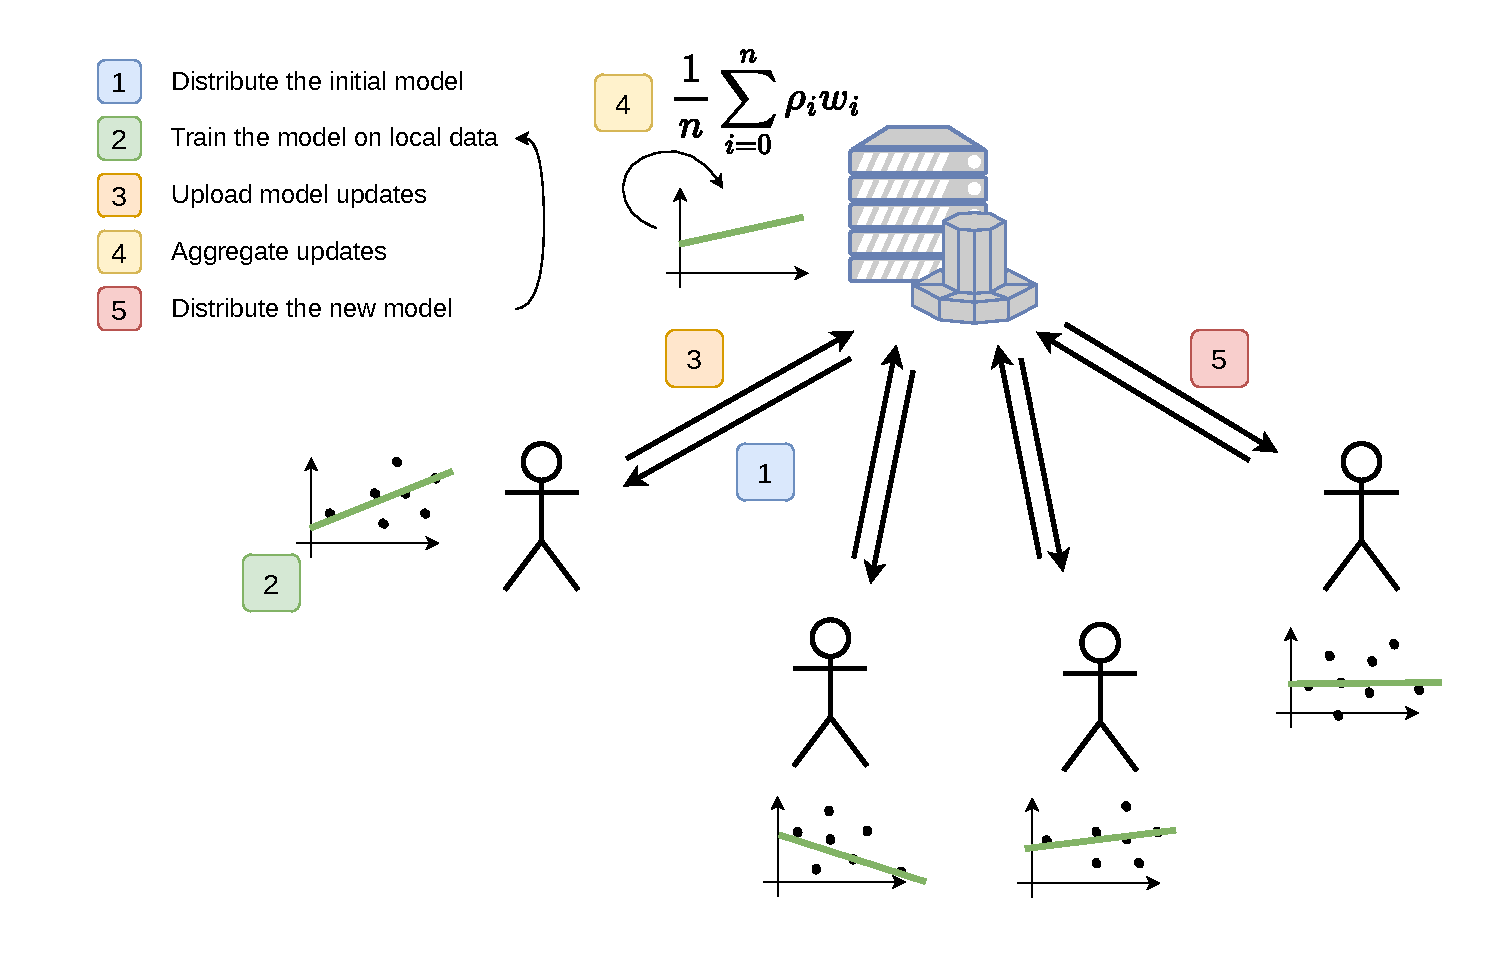
\includegraphics[width=1.1\linewidth,right]{figures/feditn/intro/fl.drawio.pdf}
            \end{figure}
        \end{column}
  \end{columns}

  \footcite*{mcmahan_Communicationefficientlearningdeep_2017}
\end{frame}

\begin{frame}{Application to Intrusion Detection}
    \vspace{-1em}

  \begin{columns}[b]
    \begin{column}{0.5\textwidth}
      \centering
      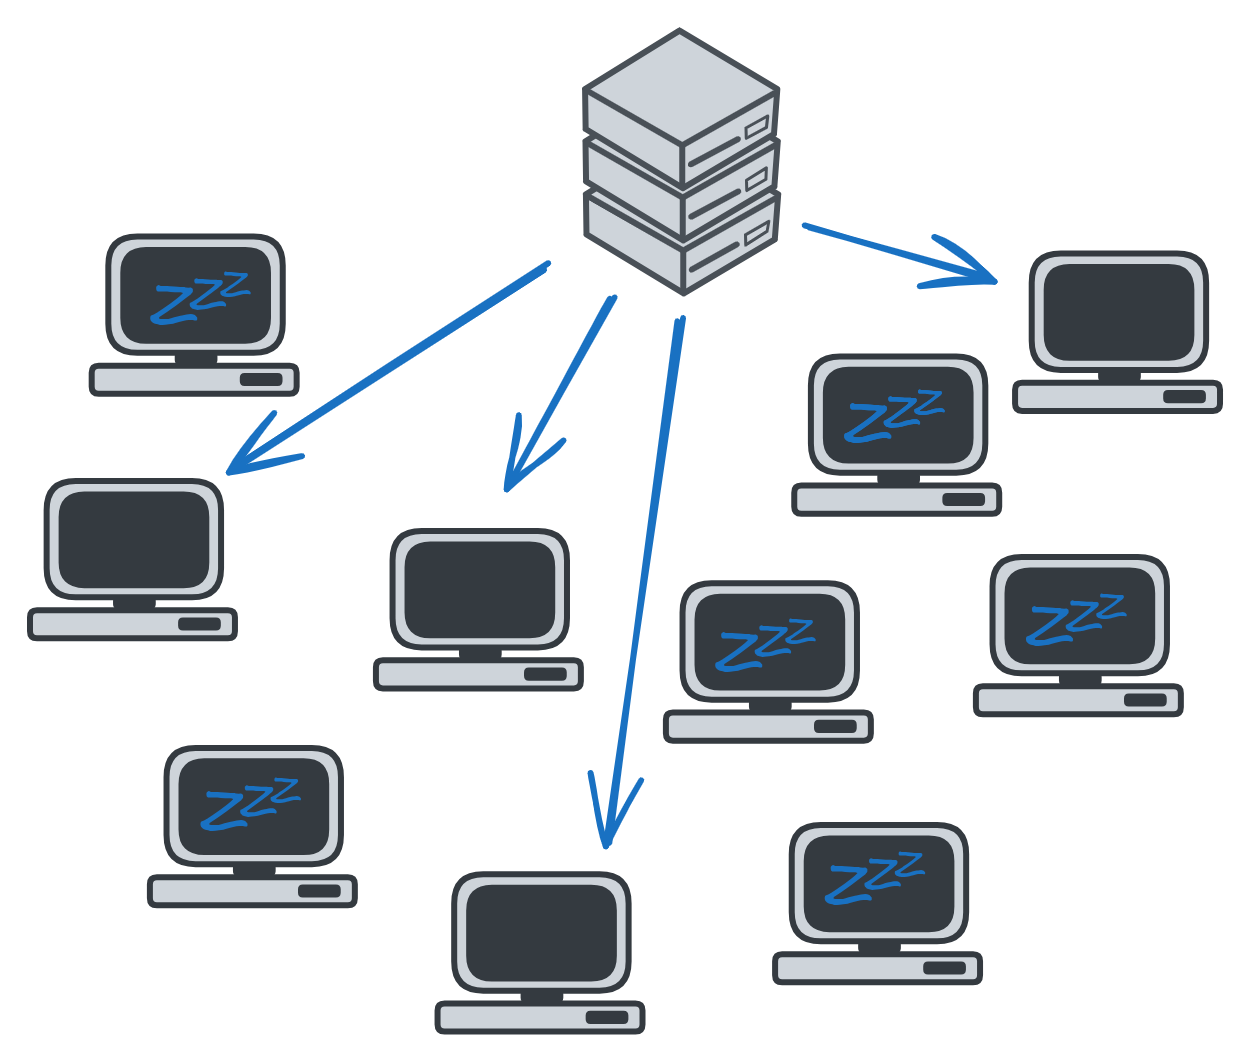
\includegraphics[width=.5\linewidth]{figures/feditn/intro/cdfl}\\
        \raggedright
        \emph{Cross-device FL}
    \end{column}
    \begin{column}{0.5\textwidth}
        \centering
        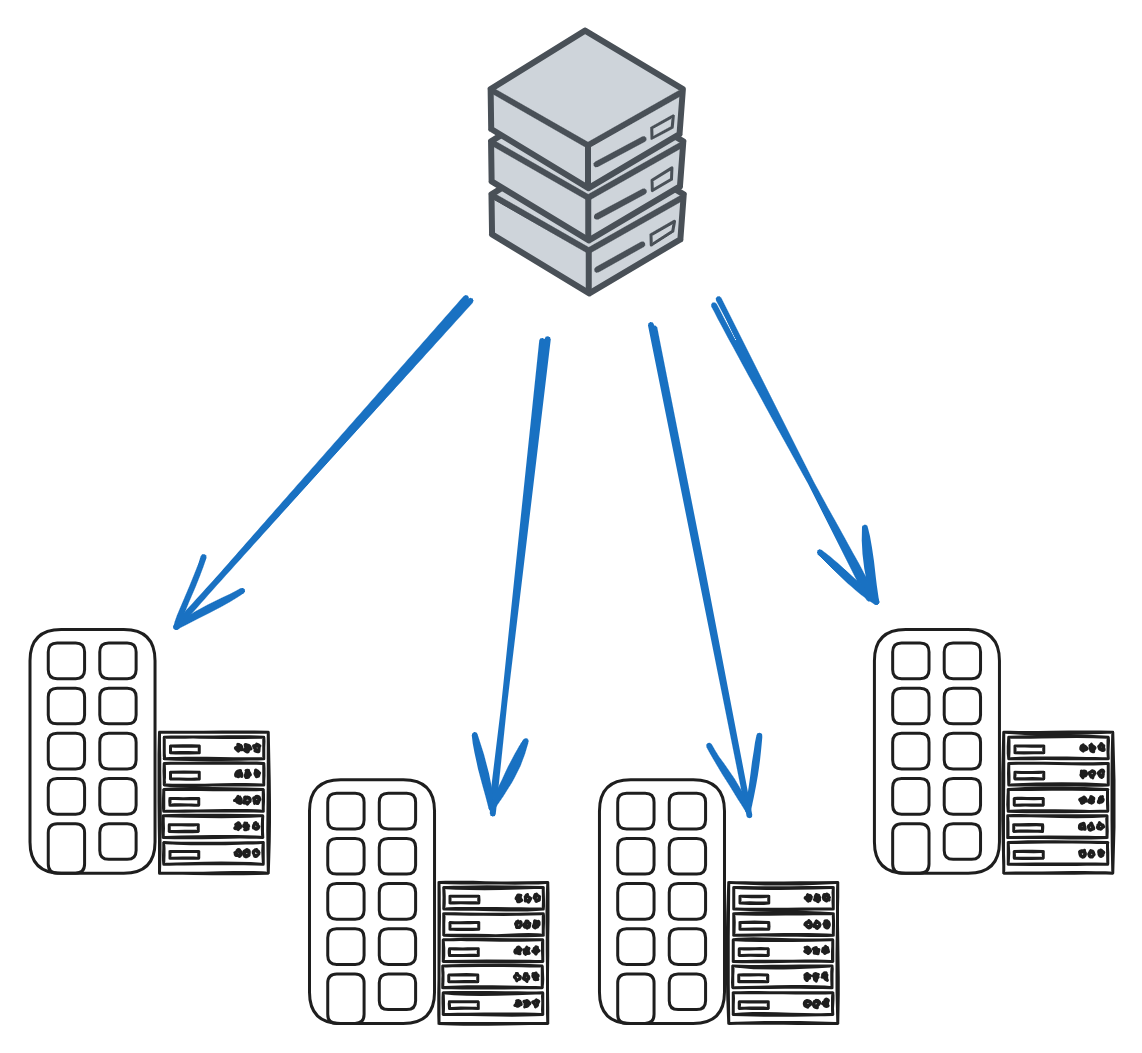
\includegraphics[width=.5\linewidth]{figures/feditn/intro/csfl}\\
        \raggedright
        \emph{Cross-silo FL}
    \end{column}
  \end{columns}
  \vspace{-1em}
  \pause
  \begin{columns}[t]
    \begin{column}{.5\textwidth}
      \begin{itemize}
        \item Learn a global from highly distributed data.
        \item Unreliable clients, limited resources.
        \pause
        \item \emph{IDS use case}: endpoint detection (\eg, EDR\footnotemark), managed IDS probes.
      \end{itemize}
    \end{column}
    \pause
    \begin{column}{.5\textwidth}
      \begin{itemize}
        \item Aggregate knowledge among few reliable clients.
        \item High computing resources.
        \pause
        \item \emph{IDS use case}: collaboration between organizations, \eg, Inter-SOCs\footnotemark.
      \end{itemize}
    \end{column}
  \end{columns}
  \only<3->{\footnotetext[1]{Endpoint Detection and Response}}
  \alt<5>{\footnotetext[2]{Security Operation Center}}{\only<3->{\blankfootnote{}}}

    \pause
  \begin{tikzpicture}[remember picture,overlay]
    \node at (current page.center)[
        rectangle, rounded corners=3pt,
        anchor=center, inner sep=10pt,
        %text width=0.45\paperwidth,
        align=center,
        fill=white, fill opacity=0.9,
        draw=sntPurple, draw opacity=0.5, very thick
      ] {
      \Large
      \textbf{Different \emph{heterogeneity} \linebreak definitions}
    };
  \end{tikzpicture}
\end{frame}

{
  \setbeamertemplate{background}{
    \begin{tikzpicture}[remember picture,overlay]
      \node at (current page.south east)[anchor=south east,inner sep=0] {
\includegraphics[width=.6\paperwidth]{assets/backgrounds/background-white}};
    \end{tikzpicture}
  }
  \begin{frame}[plain]
    \centering
    \huge\itshape
    What datasets for \emph{distributed} intrusion detection?\\[1em]
    \pause
    \normalfont
    None (:
  \end{frame}
}

\begin{frame}{Existing workarounds}
  \begin{columns}[t]
    \begin{column}{0.45\textwidth}
      \centering\large
      \emph{Partitioning datasets}~\autocite{campos_EvaluatingFederatedLearning_2022}
    \end{column}
    \begin{column}{0.1\textwidth}
      \centering
      \vs
    \end{column}
    \begin{column}{0.45\textwidth}
      \centering\large
      \emph{Homogenizing features}~\autocite{popoola_FederatedDeepLearning_2021}
    \end{column}
  \end{columns}
  \pause
  \begin{columns}[t]
    \begin{column}{0.45\textwidth}
      \begin{itemize}
        \item Risk of correlation across clients and unrealistic data points;
        \item Requires a deep understanding of the dataset;
        \item Limited by the diversity of the selected dataset.
      \end{itemize}
    \end{column}
    \begin{column}{0.1\textwidth}\end{column}
    \begin{column}{0.45\textwidth}
      \pause
      \begin{itemize}
        \item Limited by the number of available datasets;
        \item No control over the data distribution;
        \item Lack dedicated test set.
      \end{itemize}
    \end{column}
  \end{columns}

  \footcite*{campos_EvaluatingFederatedLearning_2022,popoola_FederatedDeepLearning_2021}

\end{frame}

